% \begin{filecontents}{\jobname.bib}
% @book{Dumke2001,
%     Author = {Dumke},
%     Publisher = {Vieweg},
%     Title = {Software-Engineering},
%     Year = {2001},
%     ISBN = {3-528-25355-X}}
% \end{filecontents}

% DUMKE (2001): Software-Engineering, Vieweg, ISBN 3-528-25355-X

%%%%%%%%%%%%%%%%%%%%%%%%%%%%%%%%%%%%%%%%%%%%%%%%%%%%%%%%%%%%%%%%%%%%%
% LaTeX Template: Softwaretechnik SS 2017
%
% Date: April 2017
%
%%%%%%%%%%%%%%%%%%%%%%%%%%%%%%%%%%%%%%%%%%%%%%%%%%%%%%%%%%%%%%%%%%%%%%

\documentclass[12pt]{article}
\usepackage[a4paper]{geometry}
\usepackage{framed}
\usepackage[myheadings]{fullpage}
\usepackage{fancyhdr}
\usepackage{lastpage}
\usepackage{graphicx, wrapfig, subcaption, setspace, booktabs}
% \usepackage{movie15}
\usepackage[T1]{fontenc}
\usepackage[font=small, labelfont=bf]{caption}
\usepackage[protrusion=true, expansion=true]{microtype}
\usepackage[german]{babel}
\usepackage{sectsty}
\usepackage{url, lipsum}
\usepackage[parfill]{parskip}
\usepackage{csquotes}
\usepackage[hidelinks]{hyperref}
\usepackage[acronym]{glossaries}

\usepackage[style=authoryear,backref=true]{biblatex}
\addbibresource{\jobname.bib}

\usepackage[export]{adjustbox}
\usepackage{multicol}
\usepackage{tikz}
\usepackage{float}


\makeglossaries
\glstoctrue



%-------------------------------------------------------------------------------
% Commands
%-------------------------------------------------------------------------------
\newcommand{\HRule}[1]{\rule{\linewidth}{#1}}
\input{../env}
%-------------------------------------------------------------------------------
% HEADER & FOOTER
%-------------------------------------------------------------------------------
\pagestyle{fancy}
\fancyhf{}
\setlength\headheight{15pt}
\fancyhead[L]{\newCommandName}
\fancyhead[R]{\newCommandUniversity}
\fancyfoot[R]{Seite \thepage\ von \pageref{LastPage}}

%-------------------------------------------------------------------------------
% TITLE PAGE
%-------------------------------------------------------------------------------
\begin{document}
\hypersetup{
    colorlinks,
    citecolor=black,
    filecolor=black,
    linkcolor=black,
    urlcolor=black
}


\title{ \normalsize
		\HRule{0.5pt} \\
		\LARGE \textbf{\uppercase{\newCommandDiscipline}} \\
    \smallbreak
		\small\textbf{{\newCommandTerm}}\\
		\HRule{2pt} \\ [0.5cm]
		\normalsize \today \vspace*{10\baselineskip}}

\date{}

\author{
		\newCommandName \\
		\newCommandMatriculationNumber \\
		\newCommandUniversity \\
		\newCommandFaculty
}

% \pagenumbering{gobble}

\maketitle
\thispagestyle{empty}

\newpage


\tableofcontents
\listoffigures
\newpage



%-------------------------------------------------------------------------------
% Section title formatting
\sectionfont{\scshape}
%-------------------------------------------------------------------------------

%-------------------------------------------------------------------------------
% BODY
%-------------------------------------------------------------------------------

\section{SWT - Einf"uhrung in die Softwaretechnik}

%-------------------------------------------------------------------------------
% #1
%-------------------------------------------------------------------------------

\newglossaryentry{st}{type=\acronymtype, name={ST}, description={Softwaretechnik}}
\newglossaryentry{ieee}{type=\acronymtype, name={IEEE}, description={Institute of Electrical and Electronics Engineers}}
\newglossaryentry{cmm}{name=CMM, description={Capability Maturity Model}}
\newglossaryentry{pmmm}{name=PMMM, description={Project Management Maturity Model}}

\subsection{"Ubung SWT-01}
\subsubsection*{Aufgabe:}

\begin{framed}
\textbf{Softwaretechnik allgemein}
\smallbreak
Was ist Softwaretechnik? Was wird da gelehrt? Worum geht es?
\\
Was antworten Sie?
\bigbreak
\small Bearbeitungszeit: 10 Minuten
\end{framed}
\bigbreak
\bigbreak
\subsubsection*{L"osung:}

\textbf{Der \gls{ieee}-Standard 610-1990 definiert Softwaretechnik als:}


\begin{center}
% \enquote{(1) The application of a \textbf{systematic}, \textbf{disciplined}, \textbf{quantifiable} approach to the development, operation, and maintenance of software; that is, the application of engineering to software. (2) The study of approaches as in (1)}
\enquote{The application of a  systematic\footnote{\label{foot:1}systematic - having, showing, or involving a system, method, or plan}, disciplined\footnote{\label{foot:2}disciplined - having or exhibiting discipline; rigorous}, quantifiable\footnote{\label{foot:3}quantifiable - to determine, indicate, or express the quantity of} approach to the development, operation, and maintenance of software; that is, the application of engineering to software.}
\end{center}

\bigbreak
\bigbreak

Aus dieser Definition k"onnen folgende Merkmale der \gls{st} benannt werden:
\bigbreak
\begin{itemize}
\item \gls{st} umfasst Methoden, Techniken und Instrumente zur Erstellung von auf Maschinen lauff"ahigen Programmen (Software).
\item Ziel von \gls{st} ist die Vermeidung von Fehlern, Reduktion von Aufw"anden und Erh"ohung des Kundennutzens von Software.
\item \gls{st} beinhaltet das Management von Entwicklungsprojekten f"ur Software.
\item \gls{st} umfasst die Inbetriebnahme, den Betrieb und die Wartung von Software.
\item Hierzu beschreibt \gls{st} bew"ahrte Vorgehensweisen in Modellen (Vorgehensmodelle) und definiert Qualit"atsstufen f"ur den Software-Entwicklungsprozess (\gls{cmm}, \gls{pmmm}).
\end{itemize}

\newpage

\autocite{Dumke2001} nimmt eine Einteilung in f"unf Kategorien vor:
\bigbreak
\begin{itemize}
\item \textbf{Methoden (development methods)}: \smallbreak Richtlinien, Strategien, und Technologien f"ur eine systematische, d. h. phasen- oder schrittweise Entwicklung von Software

\item \textbf{Werkzeuge (tools)}: \smallbreak rechnergest"utzte Hilfsmittel zur Software-Entwicklung und -Anwendung

\item \textbf{Ma"ssysteme (set of measurements)}: \smallbreak Menge von Software-Ma"sen zur Bewertung und Messung der Eigenschaften der zu entwickelnden Software hinsichtlich Eignung, Qualit"at und speziell des Leistungsverhaltens

\item \textbf{Standards (standards)}: \smallbreak Menge von Richtlinien f"ur die einheitliche und abgestimmte Form der Software-Entwicklung und des zu entwickelnden Software-Systems

\item \textbf{Erfahrungen (experiences)}: \smallbreak (quantifizierte) Kenntnisse "uber die Entwicklung der Software sowie das Entwicklungsergebnis selbst hinsichtlich des Einsatzes, der Qualit"at und des Nutzens (als Ingenieurwissen)
\end{itemize}


%-------------------------------------------------------------------------------
% #2
%-------------------------------------------------------------------------------
\newtheorem{defi}{Definition:}
\newpage
\subsection{"Ubung SWT-02}
\subsubsection*{Aufgabe:}

\begin{framed}
\textbf{Softwarelebenszyklus}
\smallbreak
Sie werden in einem Bewerbungsgespr"ach gebeten, die wesentlichen Teile des Softwarelebenszyklus an dem Whiteboard zu skizzieren und zu erl"autern.
\\ K"onnen Sie das?
\bigbreak
\small Bearbeitungszeit: 15 Minuten
\end{framed}
\bigbreak
\bigbreak
\subsubsection*{L"osung:}

\begin{defi}
  \textbf{Softwarelebenszyklus}
  \smallbreak
  Unter Softwarelebenszyklus versteht man die Menge aller unterscheidbaren Phasen, die das Softwareprodukt und die bei der Erstellung beteiligten Personen durchleben. Dies geht "ublicherweise von der ersten Idee bis hin zu kompletten Installation und sogar bis zur Abl"osung des Softwareproduktes.
\end{defi}
\smallbreak

% \begin{multicols}{2}
% \vfill\null
% \begin{figure}[H]
%   \centering
%   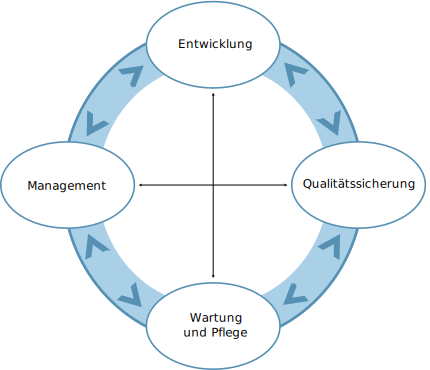
\includegraphics[width=0.5\textwidth]{./images/AbbEntwicklgProzess.png}
%   \captionsetup{name=Abb.,font=footnotesize}
%   \caption{Phasen im Software-Entwicklungsprozess (abstrakter Zyklus)}
% \end{figure}
% \vfill\null
% \columnbreak
% \textbf{Entwicklung}
% \newline
% Die Software-Entwicklung hat die Aufgabe ein Produkt zu erstellen, das die geforderten Qualit"atseigenschaften besitzt. Der Entwicklungsprozess wird im Allgemeinen in eine Reihe von Aktivit"aten aufgeteilt, deren Ergebnisse einzelne Teilprodukte sind. Solche Aktivit"aten werden nach zeitlichen, begrifflichen, technischen und/oder organisatorischen Kriterien zu Phasen zusammengefasst.
% \smallbreak
% \textbf{Management}
% \newline
% Das Software-Management ist erforderlich, um den Entwicklungsprozess zu planen, zu organisieren, zu leiten und zu kontrollieren. Entwicklung und Management im Software-Entwicklungsprozess sind vielfach voneinander abh"angig. Die Einf"uhrung neuer Methoden und Tools kann zu Ver"anderungen in den organisatorischen Strukturen f"uhren.
% \smallbreak
% \textbf{Qualit"atssicherung}
% \newline
% Die Sicherstellung einer geforderten Softwarequalit"at muss durch eine entwicklungsbegleitende Software-Qualit"atssicherung erreicht werden. Dazu sind eine Reihe von konstruktiven und analytischen Ma"ssnahmen durchzuf"uhren. Die Ma"ssnahmen der Qualit"atssicherung werden dabei sowohl von der Entwicklung (die verwendeten Methoden, Tools und Programmiersprachen erfordern bestimmte Sicherungs- und Pr"ufma"ssnahmen), als auch vom Management durch organisatorische Zuordnung der Qualit"atssicherung zum Entwicklungsprozess beeinflusst.
% % \smallbreak
% \vfill\null
% \columnbreak
%
% \textbf{Wartung und Pflege}
% \newline
% Nachdem ein Softwareprodukt zur Anwendung freigegeben wurde, beginnt die Wartung und Pflege, d. h. es gilt alle nach Inbetriebnahme auftretenden Fehler zu beseitigen, das Anwendungssystem an ver"anderte Bedingungen anzupassen und es bei Vorliegen neuer Anforderungen weiterzuentwickeln. Art und Umfang der Wartungst"atigkeiten sind auch von der Gew"ahrleistung der Qualit"atssicherung abh"angig, d. h. eine schlechte Produktqualit"at f"uhrt zwangsl"aufig zu h"aufigeren Fehleranteilen.
% \end{multicols}

% \begin{multicols}{2}
%   \begin{figure}[H]
%     \centering
%     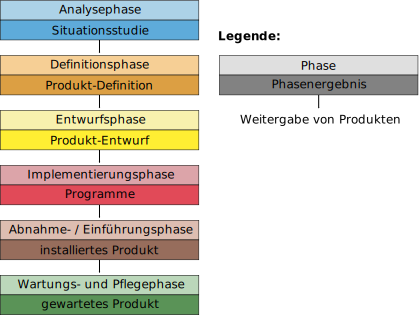
\includegraphics[width=0.5\textwidth]{./images/AbbPhaseneinteilung.png}
%     \captionsetup{name=Abb.,font=footnotesize}
%     \caption{Phaseneinteilung nach Balzert}
%   \end{figure}
% \end{multicols}






%-------------------------------------------------------------------------------
% #3
%-------------------------------------------------------------------------------
\newpage
\subsection{"Ubung SWT-03}
\subsubsection*{Aufgabe:}

\begin{framed}
\textbf{Prinzipien}
\smallbreak
Geben Sie bitte zu jedem Prinzip der Softwaretechnik (Abstraktion, Strukturierung, Hierarchisierung, Modularisierung, Standardisierung) ein Beispiel an. Wo ist Ihnen das schon begegnet und wo k"onnte das in der Softwaretechnik angewendet oder wirksam werden?
\bigbreak
\small Bearbeitungszeit: 10 Minuten
\end{framed}
\bigbreak
\bigbreak
\subsubsection*{L"osung:}
Lorem ipsum dolor sit amet, consectetur adipisicing elit, sed do eiusmod tempor incididunt ut labore et dolore magna aliqua. Ut enim ad minim veniam, quis nostrud exercitation ullamco laboris nisi ut aliquip ex ea commodo consequat. Duis aute irure dolor in reprehenderit in voluptate velit esse cillum dolore eu fugiat nulla pariatur. Excepteur sint occaecat cupidatat non proident, sunt in culpa qui officia deserunt mollit anim id est laborum.

%-------------------------------------------------------------------------------
% #4
%-------------------------------------------------------------------------------
\newpage
\subsection{"Ubung SWT-04}
\subsubsection*{Aufgabe:}

\begin{framed}
\textbf{Recherche}
\smallbreak
Recherchieren Sie bitte im Internet "uber Softwaretechnik oder Softwareengineering. Welche Bereiche interessieren Sie ganz besonders?
\bigbreak
\small Bearbeitungszeit: 30 Minuten
\end{framed}
\bigbreak
\bigbreak
\subsubsection*{L"osung:}
Lorem ipsum dolor sit amet, consectetur adipisicing elit, sed do eiusmod tempor incididunt ut labore et dolore magna aliqua. Ut enim ad minim veniam, quis nostrud exercitation ullamco laboris nisi ut aliquip ex ea commodo consequat. Duis aute irure dolor in reprehenderit in voluptate velit esse cillum dolore eu fugiat nulla pariatur. Excepteur sint occaecat cupidatat non proident, sunt in culpa qui officia deserunt mollit anim id est laborum.

%-------------------------------------------------------------------------------
% #5
%-------------------------------------------------------------------------------
\newpage
\subsection{"Ubung SWT-05}
\subsubsection*{Aufgabe:}

\begin{framed}
\textbf{Wissensfragen zur Lerneinheit}
\smallbreak
Versuchen Sie die Fragen schriftlich zu beantworten ohne noch einmal in der Lerneinheit nachzuschlagen.
\begin{enumerate}
\item An welche Best Practices erinnern Sie sich oder welche haben Sie verinnerlicht?
\item Warum ist es sinnvoll Softwarefehler fr"uh zu erkennen?
\item Was geht in Softwareprojekten typischerweise schief?
\item Kennen Sie (Standardisierungs-)Organisationen, die sich mit Software besch"aftigen?
\end{enumerate}
\bigbreak
\small Bearbeitungszeit: 15 Minuten
\end{framed}
\bigbreak
\bigbreak
\subsubsection*{L"osung:}
Lorem ipsum dolor sit amet, consectetur adipisicing elit, sed do eiusmod tempor incididunt ut labore et dolore magna aliqua. Ut enim ad minim veniam, quis nostrud exercitation ullamco laboris nisi ut aliquip ex ea commodo consequat. Duis aute irure dolor in reprehenderit in voluptate velit esse cillum dolore eu fugiat nulla pariatur. Excepteur sint occaecat cupidatat non proident, sunt in culpa qui officia deserunt mollit anim id est laborum.

%-------------------------------------------------------------------------------
% #6
%-------------------------------------------------------------------------------
\newpage
\subsection{"Ubung SWT-06}
\subsubsection*{Aufgabe:}

\begin{framed}
\textbf{Fehlerquellen}
\smallbreak
H"aufige Fehlerquellen in Softwareprojekten sind:
\bigbreak
\includegraphics[width=1.0\textwidth]{./images/ueb01-06.png}
\end{framed}
\bigbreak
\bigbreak
\subsubsection*{L"osung:}
Lorem ipsum dolor sit amet, consectetur adipisicing elit, sed do eiusmod tempor incididunt ut labore et dolore magna aliqua. Ut enim ad minim veniam, quis nostrud exercitation ullamco laboris nisi ut aliquip ex ea commodo consequat. Duis aute irure dolor in reprehenderit in voluptate velit esse cillum dolore eu fugiat nulla pariatur. Excepteur sint occaecat cupidatat non proident, sunt in culpa qui officia deserunt mollit anim id est laborum.

%-------------------------------------------------------------------------------
% #7
%-------------------------------------------------------------------------------
\newpage
\subsection{"Ubung SWT-07}
\subsubsection*{Aufgabe:}

\begin{framed}
\textbf{Phaseneinteilung}
\smallbreak
Ordnen Sie die Phasen und Ergebnisse des Softwarelebenszyklus in der richtigen Reihenfolge an.
\bigbreak
\includegraphics[width=1.0\textwidth]{./images/ueb01-07.png}
\end{framed}
\bigbreak
\bigbreak
\subsubsection*{L"osung:}
Lorem ipsum dolor sit amet, consectetur adipisicing elit, sed do eiusmod tempor incididunt ut labore et dolore magna aliqua. Ut enim ad minim veniam, quis nostrud exercitation ullamco laboris nisi ut aliquip ex ea commodo consequat. Duis aute irure dolor in reprehenderit in voluptate velit esse cillum dolore eu fugiat nulla pariatur. Excepteur sint occaecat cupidatat non proident, sunt in culpa qui officia deserunt mollit anim id est laborum.









%-------------------------------------------------------------------------------
% Literatur - Glossar - Akronyme
%-------------------------------------------------------------------------------

\clearpage
\printbibliography[heading=bibintoc]
\newpage
\printglossary[type=main]
\printglossary[type=\acronymtype]


%-------------------------------------------------------------------------------
% ENDE
%-------------------------------------------------------------------------------

\end{document}
